\documentclass[fontsize=14pt]{scrartcl}
\usepackage[utf8]{inputenc}
\usepackage[T2A]{fontenc}
\usepackage[english, russian]{babel}
\usepackage{ amssymb }
\usepackage{mathtools}
\usepackage{amsthm}
\usepackage{graphicx}
\usepackage{multicol}
\usepackage{caption}
\usepackage{listings}
\usepackage[a4paper,
            left=30mm,
            right=15mm,
            top=20mm,
            bottom=20mm,   headsep=5.5mm,
  footskip=10mm]{geometry}
\usepackage{times}
 \usepackage{setspace}
\usepackage{amsmath}
\usepackage{ dsfont }
\usepackage{indentfirst}
\usepackage{ upgreek }
\usepackage{biblatex} 
\addbibresource{sample.bib}
\usepackage{xcolor}
\usepackage{hyperref}

\graphicspath{ {./images/} }


% formatting
\onehalfspacing
\setlength{\parindent}{35pt}


\title{Магистерский диплом}

\theoremstyle{definition}
\newtheorem{definition}{Определение}[section]
\newtheorem{theorem}{Теорема}[section]
\newtheorem{lemma}[theorem]{Лемма}



\definecolor{codegreen}{rgb}{0,0.6,0}
\definecolor{codegray}{rgb}{0.5,0.5,0.5}
\definecolor{codepurple}{rgb}{0.58,0,0.82}
\definecolor{backcolour}{rgb}{0.95,0.95,0.92}

\lstdefinestyle{python}{
    backgroundcolor=\color{backcolour},   
    commentstyle=\color{codegreen},
    keywordstyle=\color{magenta},
    numberstyle=\tiny\color{codegray},
    stringstyle=\color{codepurple},
    basicstyle=\ttfamily\footnotesize,
    breakatwhitespace=false,         
    breaklines=true,                 
    captionpos=b,                    
    keepspaces=true,                 
    numbers=left,                    
    numbersep=5pt,                  
    showspaces=false,                
    showstringspaces=false,
    showtabs=false,                  
    tabsize=2,
    language=Python
}

\lstdefinestyle{output}{
showspaces=false,        
language=sh,
frame=single,        
breaklines=true,
showstringspaces=false,
}

%\lstset{style=python}



\begin{document}


\maketitle

\section{Аннотация}
Целью данной работы является изучение конструкции T-многообразий сложности 1 в терминах CDP (комбинаторных дивизориальных многогранников) и компьютерная реализация этих многообразий и некоторых их свойств. В данной работе был разработан и реализован алгоритм проверки CDP на эквивалентность, а также была реализована генерация CDP из многогранников.


\clearpage

\tableofcontents

\clearpage

\section{Введение}



\subsection{CDP и T-многообразия}

Пусть задана решетка $M$, $\square$ - многогранник с вершинами в узлах решетки, $\square^{\circ}$ - внутренность многогранника, $\partial\square$ - его граница.
\begin{definition}[Дивизориальный многогранник]
Дивизориальный многогранник на гладкой проективной кривой $Y$ относительно решетки $M$ - это кусочно-линейная вогнутая функция $\Psi = \sum^{P \in Y}\psi_P \dot P: \square \rightarrow Div_{\mathds{Q}}Y$, область определения которой - многогранник $\square$ на решетке $M$, область значений - подмножество группы $\mathds{Q}$-дивизоров на $Y$, такая что
\begin{enumerate}
	\item $deg\Psi(u) > 0$ для $u \in \square^{\circ}$
	\item $deg\Psi(u) > 0$ или $\Psi(u) \sim 0$ для $u \in \square$
	\item График $\psi_P$ имеет целочисленные вершины для всех $P \in Y$
\end{enumerate}
\end{definition}
% TODO:  добавить определение степени 


\begin{definition}[T-многообразие]
T-многообразием сложности k называется нормальное многообразие $X$ над $\mathds{C}_n$ эффективным действием тора $T \simeq (\mathds{C}^{*})^{n-k}$
\end{definition}

Дивизориальные многогранники соответствуют рациональным поляризованным T-многообразиям сложности 1 (\cite{vars}).

\begin{definition}[CDP] 
Комбинаторный дивизориальный многогранник (combinatorial divisorial polytope) относительно решетки M состоит из многогранника $\square \subset M \otimes \mathds{R}$ и кортежа $(\psi_1, \dots, \psi_n)$ кусочно-линейных вогнутых функций $\psi_i: \square \rightarrow \mathds{R}$ таких что
\begin{itemize}
	\item[1] Для всех $i$ граф $\psi_i$ - полиэдральный комплекс с целочисленными вершинами
	\item[2] $\forall u \in \square^{\circ} \sum_{i=1}^n\psi_i(u) > 0$
\end{itemize}
$\square$ называется \emph{базой} CDP
\end{definition}

Если прикрепить каждую из функций $\psi_i$ к точке $P_i$ на кривой $\mathds{P}^1$ (проективная прямая) - получится дивизориальный многогранник на $\mathds{P}^1$ (\cite{main}), что соответствует рациональным поляризованным T-многообразиям сложности 1.

\subsection{Преобразования CDP}
Пусть дан исходный CDP c набором функций $(\psi_1, \dots, \psi_n)$ и базой $\square$

\begin{definition}[Трансформация базы (transformation of the base)]
Пусть $\phi$ - линейное обратимое преобразование решетки $M$, тогда CDP с базой $\phi(\square)$ и набором функций 
$\psi_i \circ \phi^{-1}$ получен из исходного с помощью  трансформации базы.
\end{definition}

\begin{definition}[Скашивание (shearing)]
Пусть $v \in M^*, \beta_1, \dots, \beta_n \in \mathds{Z}$, тогда CDP с базой $\square$ и набором функций $u \mapsto
 \psi_i(u) + \beta_i\langle u, v \rangle, \forall u \in \square$, получен из исходного с помощью скашивания.
\end{definition}

\begin{definition}[Перенос (translation)]
Пусть $\alpha_1, \dots, \alpha_n \in \mathds{Z}
$, $\sum_{i=1}^n \alpha_i = 0$, тогда CDP с базой $\square$ и набором функций $\psi_i + \alpha_i$ получен из исходного с помощью переноса.
\end{definition}

\subsection{Эквивалентность}
\begin{definition}[Эквивалентные CDP]
CDP, полученный из исходного с помощью преобразований скашивания, переноса и трансформации базы, примененных в любой последовательности и в любых количествах, эквивалентен исходному.
\end{definition}
Геометрический смысл определения эквивалентности заключается в следующем: если для CDP $\psi$ прикрепить точки $P_i \in \mathds{P}^1$ - получится дивизориальный многогранник на $\mathds{P}^1$, который соответствует рациональному поляризованному T-многообразию сложности 1. Эквивалентные CDP задают эквивариантно изоморфные T-многообразия сложности 1 при условии "правильного" выбора точек $P_i$.

\begin{definition}[Грань высоты 1]
	Грань $F$ многогранника $P \in (M \times \mathds{Z}) \otimes \mathds{R}$ является гранью высоты 1, если существует вектор $u \in M^* \times \mathds{Z}$ такой что $\langle v, u\rangle = 1$ для всех $v \in F$
\end{definition}

\begin{definition}[Свойство Фано]
CDP обладает свойством Фано, если он эквивалентен какому-то CDP с базой $\square$ и функциями $\psi_1, \dots \psi_n$ для которого существуют коэффициенты $a_1, \dots, a_n$ такие что 
\begin{enumerate}
	\item $0 \in \square^{\circ}$
	\item $\sum_{i=1}^n a_i = -2$
	\item Для всех i $\psi_i(0) + a_i + 1 > 0$, и каждая грань $\Gamma(\psi_i + a_i + 1)$ - грань высоты 1
	\item Для каждой грани $F$ многогранника $\square$ не являющейся гранью высоты 1 верно $\sum_{i=1}^n \psi_i \equiv 0$ на всей $F$
\end{enumerate}
\end{definition}

Все свойства определения Фано сохраняются для эквивалентных CDP при условии что трансформация базы оставляет начало координат внутри базы (\cite{main}).
Внутри класса рациональных поляризованных T-многообразий сложности 1, CDP, удовлетворяющие свойству Фано, соответствуют каноническим T-многообразиям Горенштейна-Фано с анти-канонической поляризацией.
\subsection{Генерация CDP из многогранников}
Рассмотрим многогранник $P \in (M \times \mathds{Z}) \otimes \mathds{R}$ с вершинами на решетке $M \times \mathds{Z}$. Из него можно получить CDP. Пусть $\pi_1$ - проекция на $M \otimes \mathds{R}$, $\pi_2$ - проекция на $\mathds{R}$. Возьмем $\square = \pi_1(P)$ и $\psi_1, psi_2: \square \rightarrow \mathds{R}$: 
$ \psi_1(u) = max(\pi_2(\pi_1^{-1}(u) \cap P))$, $\psi_2(u) = -min(\pi_2(\pi_1^{-1}(u) \cap P))$. Таким образом, из любого многогранника на решетке можно получить CDP c двумя функциями. И наоборот, из любого CDP с двумя функциями можно получить многогранник на решетке.

\begin{figure}[!htb]
\minipage{0.32\textwidth}
  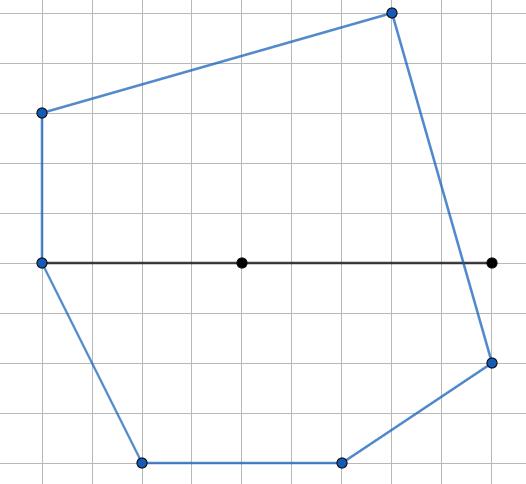
\includegraphics[width=\linewidth]{poly1.png}
  \caption{Многогранник}\label{fig:awesome_image1}
\endminipage\hfill
\minipage{0.32\textwidth}
  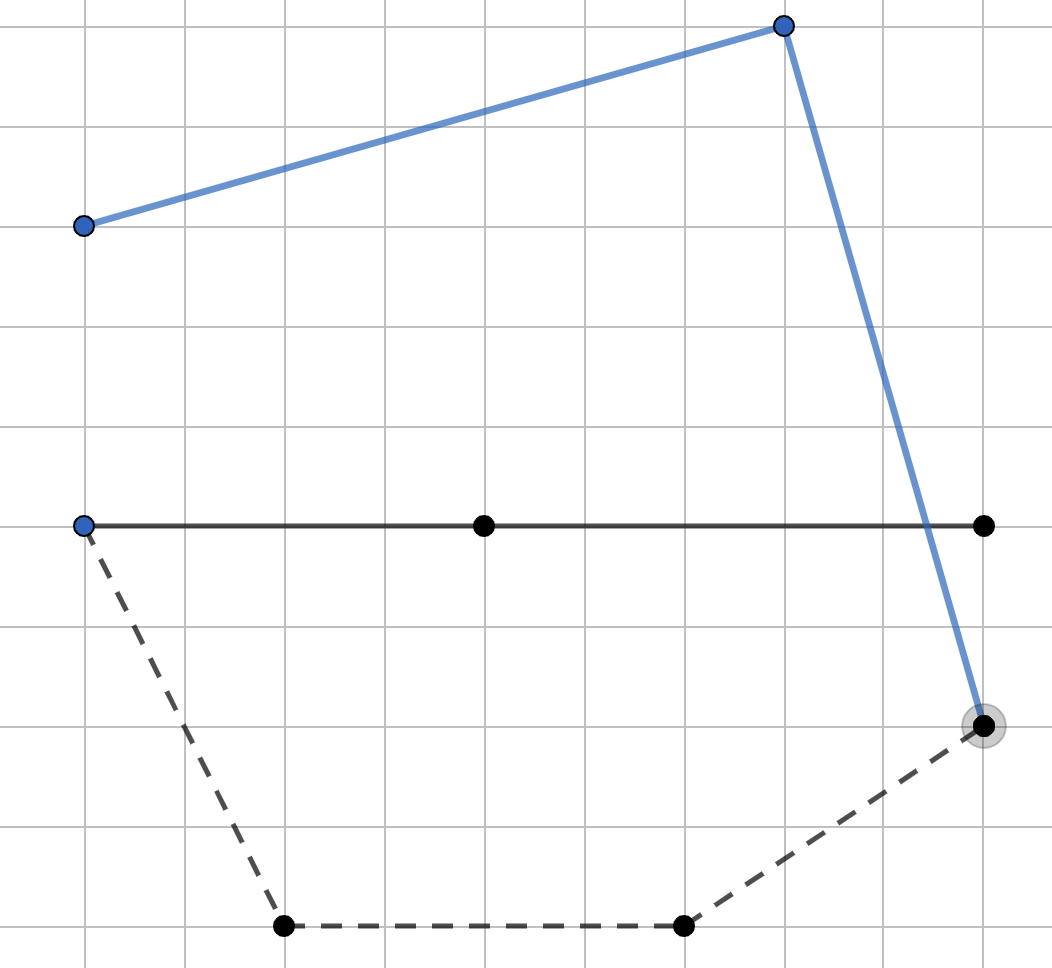
\includegraphics[width=\linewidth]{poly2.png}
  \caption{$\square = \pi_1(P)$}\label{fig:awesome_image2}
\endminipage\hfill
\minipage{0.32\textwidth}%
  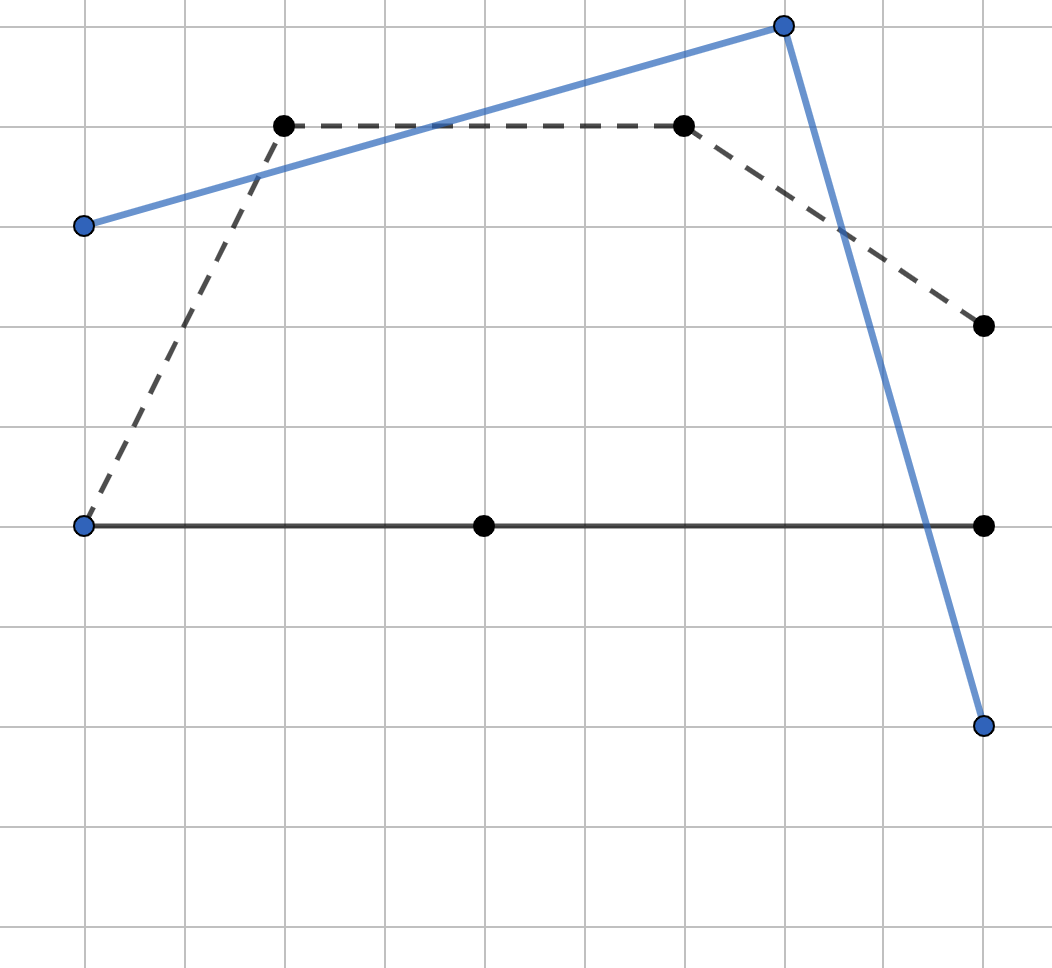
\includegraphics[width=\linewidth]{poly3.png}
  \caption{CDP}\label{fig:awesome_image3}
\endminipage
\caption{Пример (На втором и третьем рисунках пунктирная линия - грани, которые вошли в график  $\psi_1$, голубая линия - грани, которые вошли в график $\psi_2$)}
\end{figure}

\begin{definition}[Торический CDP]
CDP называется торическим, если он эквивалентен CDP с ровно двумя функциями
\end{definition}

Любой торический CDP можно получить из многогранника с помощью алгоритма, описанного выше.

Торический CDP является Фано тогда и только тогда, когда соответствующий ему многогранник изоморфен рефлексивному.
\section{Компьютерная реализация CDP}
Весь код реализован на Python3 и представлен в Приложении, а также доступен по ссылке \href{https://github.com/irina-batmanova/masters}. В реализации используется класс Polyhedron из библиотеки sagemath.

Класс CDP имеет два поля - base (класс Polyhedron из sage) и $psi\_list$ - список объектов класса PiecewiseAffineFunction. 
Класс PiecewiseAffineFunction - реализация кусочно-линейной функции, класс имеет одно поле - $affine\_pieces$, список объектов класса AffineFunction. Класс AffineFunction - реализация линейной функции, содержит два поля - domain (класс Polyhedron из sage, это область, на которой задана функция) и coefs - список коэффициентов в формате $[a_0, a_1, \dots, a_{k-1}]$, тогда функция имеет вид $x_k = a_0 + a_1 x_1 + \dots + a_{k-1} x_{k-1}$

CDP - сложный объект, нужно соблюсти множество условий, чтобы сконструировать правильный CDP, поэтому в конструкторе проверяется корректность поданных на вход данных. 

\noindent{Пример корректного CDP:}

\noindent{Пример взят из статьи \cite{main}}

\begin{lstlisting}[language=Python, label={correct}, style=python] 
base = Polyhedron(vertices=[[-1], [1]])
# y = 1 + x, x \in [-1, 0]
f_11 = AffineFunction([1, 1], Polyhedron(vertices=[[-1], [0]]))
# y = 1 - x, x \in [0, 1]
f_12 = AffineFunction([1, -1], Polyhedron(vertices=[[0], [1]]))
f_1 = PiecewiseAffineFunction([f_11, f_12])
# y = 1/2x + 1/2, x \in [-1, 1]
f_2 = PiecewiseAffineFunction([AffineFunction([1 / 2, 1 / 2], Polyhedron(vertices=[[-1], [1]]))])
cdp = CDP([f_1, f_2], base)
print(cdp)
\end{lstlisting}

\begin{figure}[h]
\centering
  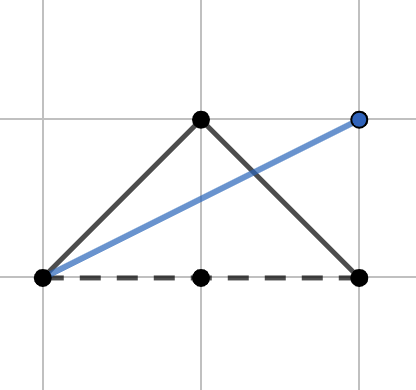
\includegraphics{correct_cdp.png}
  \caption{Корректный CDP}\label{correntcdp}
\end{figure}

\noindent{Программа выведет:}
\begin{lstlisting}[style=output]
CDP object, psi list:
Piecewise affine function:
Affine function 1 + x_1 with domain [(-1), (0)]
Affine function 1 - x_1 with domain [(0), (1)]

Piecewise affine function:
Affine function 0.5 + 0.5x_1 with domain [(-1), (1)],

base: (A vertex at (-1), A vertex at (1))
\end{lstlisting}

\noindent{Пример некорректного CDP (сумма $\psi_i$ отрицательная в одной из точек базы):}
\begin{figure}[h]
\centering
  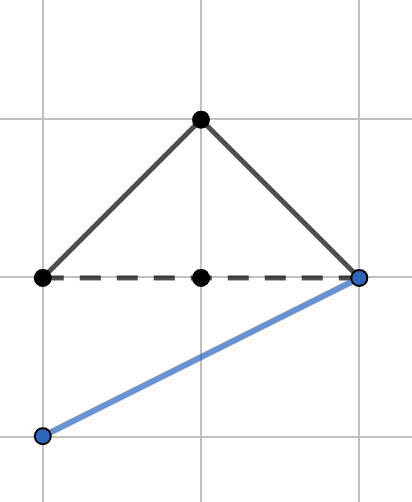
\includegraphics{bad_cdp.png}
  \caption{Некорректный CDP}\label{correntcdp}
\end{figure}

\begin{lstlisting}[language=Python,style=python]
base = Polyhedron(vertices=[[-1], [1]])
# y = x, x \in [-1, 0]
f_11 = AffineFunction([0, 1], Polyhedron(vertices=[[-1], [0]]))
# y = -x, x \in [0, 1]
f_12 = AffineFunction([0, -1], Polyhedron(vertices=[[0], [1]]))
f_1 = PiecewiseAffineFunction([f_11, f_12])
# y = -1/2 + 1/2x, x \in [-1, 1]
f_2 = PiecewiseAffineFunction([AffineFunction([-1 / 2, 1 / 2], Polyhedron(vertices=[[-1], [1]]))])
cdp = CDP([f_1, f_2], base)	
\end{lstlisting}

\noindent{Программа выведет:}
\begin{lstlisting}[style=output]
Traceback (most recent call last):
  File "/Users/irinanifantova/mipt/masters/cdp/./test_cdp_validity.py", line 65, in <module>
    test.test_not_valid_cdp()
  File "/Users/irinanifantova/mipt/masters/cdp/./test_cdp_validity.py", line 30, in test_not_valid_cdp
    cdp = CDP([f_1, f_2], base)
  File "/Users/irinanifantova/mipt/masters/cdp/cdp.py", line 27, in __init__
    raise ValueError(
ValueError: Not a valid CDP - sum of psi is -2.0 on A vertex at (-1)
\end{lstlisting}


\subsection{Преобразования CDP}

\noindent{Применим скашивание к CDP из примера \ref{correct}:} с коэффициентом -1 для первой функции и 1 для второй, с вектором (-1).

\begin{lstlisting}[language=Python,style=python]
cdp = CDP([f_1, f_2], base)
cdp.shear([-1, 1], [-1])
print(cdp)
\end{lstlisting}

\noindent{Программа выведет:}

\begin{lstlisting}[style=output]
CDP object, psi list:
Piecewise affine function:
Affine function 1 + 2x_1 with domain [(-1), (0)]
Affine function 1 with domain [(0), (1)]

Piecewise affine function:
Affine function 0.5 - 0.5x_1 with domain [(-1), (1)],

base: (A vertex at (-1), A vertex at (1))
\end{lstlisting}

\begin{figure}[!htb]
\minipage{0.45\textwidth}
  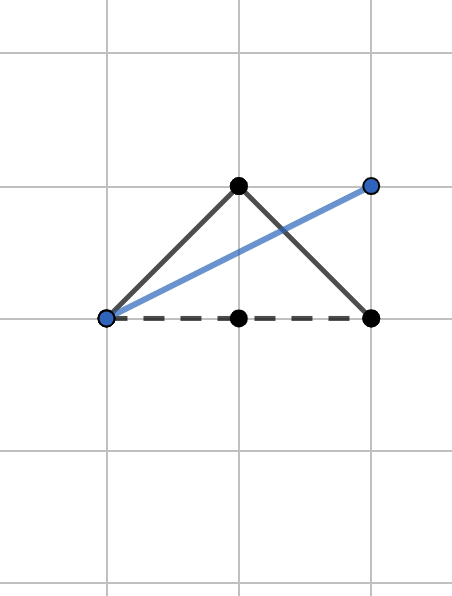
\includegraphics[width=\linewidth]{cdp.png}
  \caption{Исходный CDP}\label{fig:awesome_image1}
\endminipage\hfill
\minipage{0.45\textwidth}
  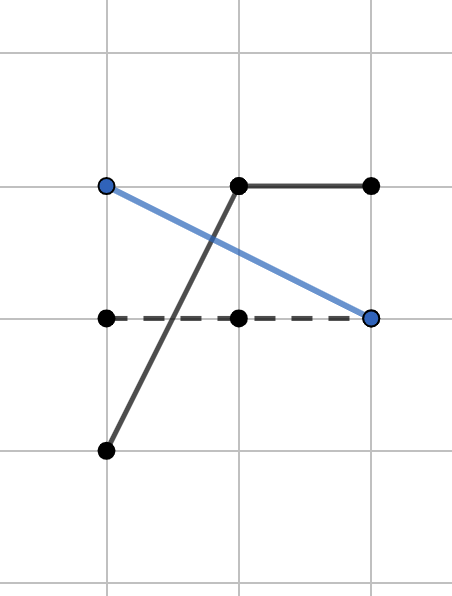
\includegraphics[width=\linewidth]{shear.png}
  \caption{После скашивания}\label{fig:awesome_image2}
\endminipage\hfill
\end{figure}

\noindent{Применим сдвиг с коэффициентами 1, -1 к результату предыдущего преобразования:}

\begin{lstlisting}[language=Python,style=python]
cdp.translate([1, -1])
print(cdp)
\end{lstlisting}

\noindent{Результат:}
\begin{lstlisting}[style=output]
CDP object, psi list:
Piecewise affine function:
Affine function 2 + 2x_1 with domain [(-1), (0)]
Affine function 2 with domain [(0), (1)]

Piecewise affine function:
Affine function -0.5 - 0.5x_1 with domain [(-1), (1)],

base: (A vertex at (-1), A vertex at (1))
\end{lstlisting}

\noindent{Применим трансформацию базы - зеркальное отображение относительно начала координат - к результату предыдущего преобразования:}

\begin{lstlisting}[language=Python,style=python]
A = matrix(ZZ, [[-1]])
phi = linear_transformation(A)
cdp.transform_base(phi)
print(cdp)
\end{lstlisting}

\noindent{Результат:}
\begin{lstlisting}[style=output]
CDP object, psi list:
Piecewise affine function:
Affine function 2 - 2x_1 with domain [(0), (1)]
Affine function 2 with domain [(-1), (0)]

Piecewise affine function:
Affine function -0.5 + 0.5x_1 with domain [(-1), (1)],

base: (A vertex at (-1), A vertex at (1))
\end{lstlisting}


\begin{figure}[!htb]
\minipage{0.45\textwidth}
  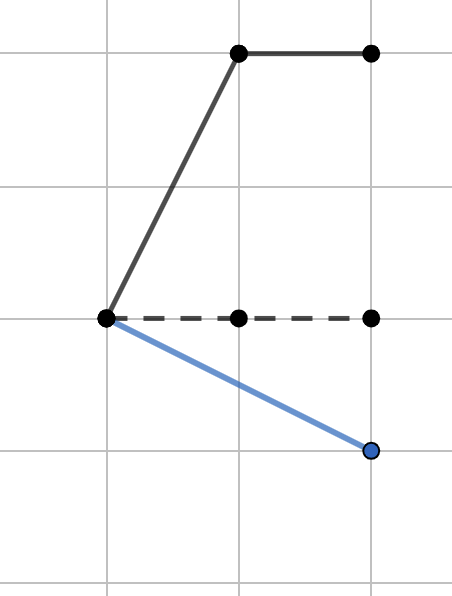
\includegraphics[width=\linewidth]{translate.png}
  \caption{После переноса}\label{fig:awesome_image1}
\endminipage\hfill
\minipage{0.45\textwidth}
  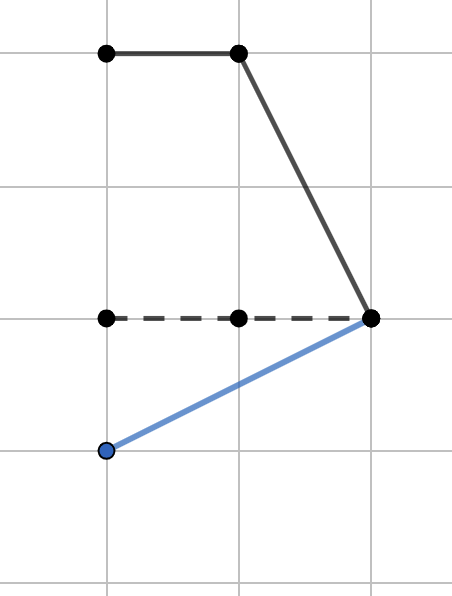
\includegraphics[width=\linewidth]{transformbase.png}
  \caption{После трансформации}\label{fig:awesome_image2}
\endminipage\hfill
\end{figure}


\subsection{Алгоритм проверки эквивалентности}
Считаем, что трансформация базы всегда происходит только 1 раз, и это первая операция в цепочке преобразований (ниже будет доказано, почему такое предположение корректно).
\\
Введем операцию обобщенного скашивания:

\begin{definition}[Обобщенное скашивание]
пусть $\sum_{i=1}^n v_i = 0$, тогда CDP с базой $\square$ и набором функций $u \mapsto \psi_i(u) + \langle u, v_i \rangle$ получен из CDP $(\square, \psi_1, \dots, \psi_n)$ с помощью обобщенного скашивания.
\end{definition}

Полный код алгоритма находится в Приложении в разделе \pageref{cdppy}


\subsubsection{Описание}

Пусть $CDP_1 = (\square, (\psi_1, \dots, \psi_n)$, $CDP_2 = (\square^{'}, (\psi^{'}_1, \dots, \psi^{'}_n)$, проверим их на эквивалентность:
\begin{itemize}
\item[1] Выберем нумерацию вершин в $\square'$. Если уже перебрали все возможные нумерации	- завершаем алгоритм, CDP не эквивалентны.
\item[2] Найдем такую матрицу $A$, которая переводит $\square$ в $\square'$ с учетом нумерации вершин, найдем матрицу обратного преобразования - $A^{-1}$. Если не удалось найти $A$ или $A^{-1}$ - переходим к шагу 1 (выбираем другую нумерацию вершин). Применим $A^{-1}$ к $\psi_1, ..., \psi_n$, получим $\upchi_1 := \psi_1\phi^{-1}, ..., \upchi_n := \psi_n\phi^{-1}$.
\item[3] Для каждой $\upchi_i$ найдем множество $S_i = \{j: \upchi_i \sim \psi^{'}_j\}$ - множество ииндексов функций $\psi^{'}_j$, имеющих такие же области линейности (иллюстрация \ref{eqclasses}). С помощью переноса или скашивания нельзя из линейной функции получить кусочно-линейную и наоборот, поэтому если для каких-то $\upchi_i$ или $\psi^{'}_j$ не нашлось соответствия - возвращаемся на шаг 1, выбираем другую нумерацию вершин базы.
\begin{figure}[!htb]
\centering
  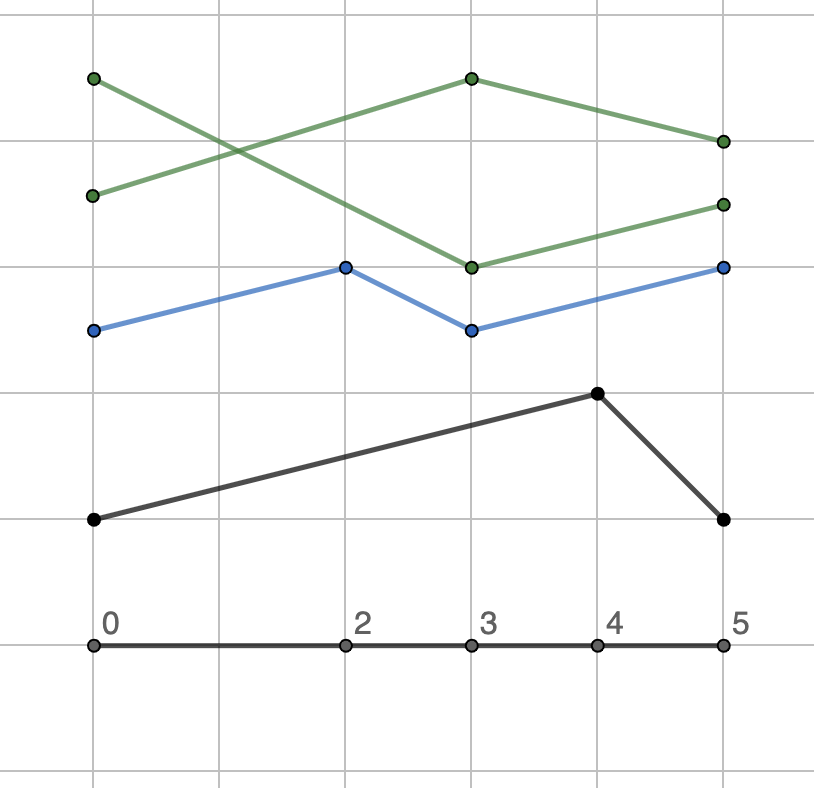
\includegraphics[scale=0.5]{eqclasses.png}
  \caption{Зеленые функции имеют области линейности $[[0, 3], [3, 5]]$, голубая - $[[0, 2], [2, 3], [3, 5]]$, черная - $[[0, 4], [4, 5]]$. Зеленые функции имеют одинаковые области линейности.}\label{eqclasses}
\end{figure}

\item[4] Каждая функция представляется в виде набора коэффициентов $a_0, a_1, \dots, a_m$, где $a_0$ - свободный коэффициент (константа), а $a_1, \dots, a_m$ - коэффициенты перед переменными $x_1, \dots, x_m$. 
Выберем $\sigma$ - перестановку функций $\upchi_i$ c учетом классов эквивалентности (то есть $\sigma(i) \in S_i$ - $\upchi_{\sigma(i)}$ и $\psi^{'}_i$ имеют одинаковые области линейности). Если все перестановки уже перебрали - переходим к шагу 1. Пусть у $\upchi_{\sigma(i)}$ коэффициенты $a_{i0}, a_{i1}, \dots, a_{im}$, у $\psi^{'}_i$ - $b_{i0}, b_{i1}, \dots, b_{im}$, тогда если $\sum_{i=1}^{n}(b_{i0} - a_{i0}) = 0$, то существует перенос, позволяющий коэффициенты $a_{i0}$ перевести в $b_{i0}$ (перенос по определению меняет только свободные коэффициенты). Если $\sum_{i=1}^{n}(b_{i0} - a_{i0}) = 0$ - обозначаем функции с коэффициентами $b_{i0}, a_{i1}, \dots, a_{im}$ как $\upchi^{'}_i$ и переходим к шагу 5, если нет - повторяем шаг 4 для другой перестановки. 

\item[5] Для каждой пары функций $\upchi^{'}_i$, $\psi^{'}_i$ пытаемся найти вектор $v_i$, такой что $\upchi^{'}_i(u) + \langle u, v_i \rangle = \psi^{'}_i(u)$, при этом для всех областей линейности должен получиться одинаковый вектор. Если для всех пар функций получилось найти такой вектор и $\sum_{i=1}^n v_i = 0$ - CDP эквивалентны (поскольку удалось найти последовательность из трансформации базы, переноса и обобщенного скашивания, переводящую CDP1 в CDP2), если нет - возвращаемся к пункту 4, выбирая другую перестановку.
\end{itemize}

\subsubsection{Примеры работы:}

\noindent{Пример из статьи \cite{main}. В предыдущем разделе (преобразования CDP) CDP2 был получен из CDP1 с помощью цепочки преобразований.}

\begin{lstlisting}[language=Python,style=python]
base1 = Polyhedron(vertices=[[-1], [1]])
# y = 1 + x, x \in [-1, 0]
f_11 = AffineFunction([1, 1], Polyhedron(vertices=[[-1], [0]]))
# y = 1 - x, x \in [0, 1]
f_12 = AffineFunction([1, -1], Polyhedron(vertices=[[0], [1]]))
f_1 = PiecewiseAffineFunction([f_11, f_12])
# y = 1/2 + 1/2x, x \in [-1, 1]
f_2 = PiecewiseAffineFunction([AffineFunction([1 / 2, 1 / 2], Polyhedron(vertices=[[-1], [1]]))])
cdp1 = CDP([f_1, f_2], base1)
base2 = Polyhedron(vertices=[[-1], [1]])
# y = 2, x \in [-1, 0]
y_11 = AffineFunction([2, 0], Polyhedron(vertices=[[-1], [0]]))
# y = 2 - 2x, x \in [0, 1]
y_12 = AffineFunction([2, -2], Polyhedron(vertices=[[0], [1]]))
y_1 = PiecewiseAffineFunction([y_11, y_12])
# y = -1/2 + 1/2x, x \in [-1, 1]
y_2 = PiecewiseAffineFunction([AffineFunction([-1 / 2, 1 / 2], Polyhedron(vertices=[[-1], [1]]))])
cdp2 = CDP([y_1, y_2], base2)
print(cdp1.equal(cdp2))
print(cdp2.equal(cdp1))
\end{lstlisting}


\begin{lstlisting}[style=output]
True
True
\end{lstlisting}

\noindent{Пример для большей размерности:}
\begin{lstlisting}[language=Python,style=python]
base1 = Polyhedron(vertices=[[1, 0], [0, -1], [-1, 0], [0, 1]])
f_11 = AffineFunction([1, -1, -1], Polyhedron(vertices=[[0, 0], [1, 0], [0, 1]]))
f_12 = AffineFunction([1, -1, 1], Polyhedron(vertices=[[0, 0], [1, 0], [0, -1]]))
f_13 = AffineFunction([1, 1, -1], Polyhedron(vertices=[[0, 0], [-1, 0], [0, 1]]))
f_14 = AffineFunction([1, 1, 1], Polyhedron(vertices=[[0, 0], [-1, 0], [0, -1]]))
f_1 = PiecewiseAffineFunction([f_11, f_12, f_13, f_14])
f_21 = AffineFunction([1, 0, 0], Polyhedron(vertices=[[0, 1], [1, 0], [0, -1]]))
f_22 = AffineFunction([1, 1, 1], Polyhedron(vertices=[[0, 0], [0, -1], [-1, 0]]))
f_23 = AffineFunction([1, 1, -1], Polyhedron(vertices=[[0, 0], [-1, 0], [0, 1]]))
f_2 = PiecewiseAffineFunction([f_21, f_22, f_23])
cdp1 = CDP([f_1, f_2], base1)
cdp2 = deepcopy(cdp1)
cdp2.shear([1, -1], [1, 1])
phi = linear_transformation(matrix(ZZ, [[-1, 0], [0, -1]]))
cdp2.transform_base(phi)
print(cdp1.equal(cdp2))
print(cdp2.equal(cdp1))
\end{lstlisting}

\begin{lstlisting}[style=output]
True
True
\end{lstlisting}

\noindent{Пример не эквивалентных CDP:}
\begin{lstlisting}[language=Python,style=python]
base1 = Polyhedron(vertices=[[-1], [1]])
# y = 1 + x, x \in [-1, 0]
f_11 = AffineFunction([1, 1], Polyhedron(vertices=[[-1], [0]]))
# y = 1 - x, x \in [0, 1]
f_12 = AffineFunction([1, -1], Polyhedron(vertices=[[0], [1]]))
f_1 = PiecewiseAffineFunction([f_11, f_12])
# y = 1/2 + 1/2x, x \in [-1, 1]
f_2 = PiecewiseAffineFunction([AffineFunction([1 / 2, 1 / 2], Polyhedron(vertices=[[-1], [1]]))])
cdp1 = CDP([f_1, f_2], base1)
base2 = Polyhedron(vertices=[[-1], [1]])
# y = 2, x \in [-1, 0]
y_11 = AffineFunction([2, 0], Polyhedron(vertices=[[-1], [0]]))
# y = 2 - x, x \in [0, 1]
y_12 = AffineFunction([2, -1], Polyhedron(vertices=[[0], [1]]))
y_1 = PiecewiseAffineFunction([y_11, y_12])
# y = -1/2 + 1/2x, x \in [-1, 1]
y_2 = PiecewiseAffineFunction([AffineFunction([-1 / 2, 1 / 2], Polyhedron(vertices=[[-1], [1]]))])
cdp2 = CDP([y_1, y_2], base2)
print(cdp1.equal(cdp2))
print(cdp2.equal(cdp1))
\end{lstlisting}

\begin{lstlisting}[style=output]
False
False
\end{lstlisting}


\subsubsection{Доказательство корректности}

\begin{theorem}
	Любую цепочку преобразований CDP можно представить в виде трех последовательных преобразований: трансформации базы, переноса и обобщенного скашивания.
\end{theorem}
\begin{proof}
	Все трансформации базы, присутствующие в цепочке преобразований, можно перенести в ее начало по Лемме \ref{transform_is_first}. После этого все трансформации можно объединить в одну по Лемме \ref{unite}. Далее можно поменять местами переносы и скашивания так, чтобы все переносы происходили последовательно следом за трансформацией базы по Лемме \ref{reorder}. Оставшиеся операции скашивания можно объединить в одно обобщенное скашивание по Лемме \ref{joinshear}.
\end{proof}

\begin{theorem}
	Если удалось найти цепочку преобразований, переводящую CDP1 в CDP2 и состоящую из трех последовательных преобразований - трансформации базы, переноса и обобщенного скашивания - то эти CDP эквивалентны.
\end{theorem}
\begin{proof}
	Нужно доказать, что существует цепочка, состоящая из трансформаций базы, переносов и обычных скашиваний, переводящая CDP1 в CDP2, то есть нужно доказать, что обощенное скашивание можно представить в виде композиции обычных. Это доказывается в лемме \ref{usual}.
\end{proof}

\begin{lemma}
\label{transform_is_first}
	Трансформацию базы можно всегда считать первой в цепочке преобразований
\end{lemma}
\begin{proof}
	Пусть $CDP_1\ (\square, \psi_1, ..., \psi_n)$ переводится в $CDP_2\ (\square^{'}, \psi_1^{'}, ..., \psi_n^{'})$ с помощью цепочки преобразований $BC$, где $B$ - операция скашивания, $C$ - трансформация базы. Покажем, что тогда существует другая цепочка преобразований - $C^{'}B^{'}$, где  $C^{'}$ - трансформация базы, $B^{'}$ - операция скашивания, - которая также переводит $CDP_1$ в $CDP_2$.
\\
$\psi_i(u) \xrightarrow[]{C^{'}B^{'}} \psi_i^{'}(u_{new}) = \psi_i(\phi^{-1}(u_{new})) + \beta_i\langle u_{new}, v\rangle $
\\
$\psi_i(u) \xrightarrow[]{B} \psi_i(u) + \beta_i \langle u, v_1 \rangle$, положим $v_1 = \phi(v)$, тогда $\psi_i(u) \xrightarrow[]{B} \psi_i(u) + \beta_i\langle u, \phi(v)\rangle$, теперь применим трансформацию $C$: 
$\psi_i(u) \xrightarrow[]{BC} \psi_i(\phi^{-1}(u_{new})) + \beta_i\langle \phi^{-1}(u_{new}), \phi(v)\rangle = \psi_i(\phi^{-1}(u_{new})) + \beta_i\langle u_{new}, v\rangle = \psi_i^{'}(u_{new})$, то есть цепочки преобразований $BC$ и $C^{'}B^{'}$ дают одинаковый результат

Аналогично для операции переноса (translation)
\end{proof}

\begin{lemma}
\label{unite}
Можно считать, что трансформация базы происходит только 1 раз в цепочке преобразований
\end{lemma}
\begin{proof}
	Все трансформации базы можно перенести в начало цепочки по предыдущему пункту, а композиция линейных обратимых преобразований также является линейным обратимым преобразованием, поэтому можно заменить композицию трансформаций на единственную трансформацию базы.

\end{proof}

\begin{lemma}
\label{reorder}
	Перенос и скашивание можно менять местами
\end{lemma}
\begin{proof}
	$\psi_i(u) + \beta_i\langle u, v\rangle + \alpha_i = \psi_i(u) + \alpha_i + \beta_i\langle u, v\rangle$
\end{proof}

\begin{lemma}
	Два переноса можно объединить в один
\end{lemma}

\begin{proof}
$\psi_i + \alpha_i + \alpha^{'}_i$, $\sum_{i=1}^n\alpha_i = 0$, $\sum_{i=1}^n\alpha^{'}_i = 0$ - значит и $\sum_{i=1}^n(\alpha_i + \alpha^{'}_i) = 0$, тогда $\psi_i + \alpha^{''}_i$, $\alpha^{''}_i = \alpha_i + \alpha^{'}_i$ - корректный перенос.	
\end{proof}

\begin{lemma}
\label{joinshear}
	Два скашивания можно объединить в одно обобщенное скашивание
\end{lemma}
\begin{proof}
	Пусть $\phi_i(u) = \psi_i(u) + \beta_i\langle u, v \rangle$, $\upchi_i(u) = \phi_i(u) + \beta^{'}_i\langle u, v^{'} \rangle$, тогда $\upchi_i(u) = \psi_i(u) + \beta_i\langle u, v \rangle + \beta^{'}_i\langle u, v^{'} \rangle = \psi_i(u) + \langle u, w \rangle$
$\sum_{i=1}^{n} \beta_i = 0$, 
$\sum_{i=1}^{n} \beta^{'}_i = 0$, 
тогда $\sum_{i=1}^{n} \beta_i\langle u, v\rangle= 0$ и $\sum_{i=1}^{n} \beta^{'}_i\langle u, v^{'}\rangle= 0$, 
а значит $\sum_{i=1}^{n} w = 0$, то есть $\upchi_i$ можно получить из $\phi_i$ с помощью операции обощенного скашивания.
\end{proof}

\begin{lemma}
\label{usual}
	Любое обобщенное скашивание можно представить в виде суммы обычных
\end{lemma}

\begin{proof}
	Пусть $v_1, \dots, v_n$ - обобщенное скашивание. Покажем, что $v_i$ можно представить в виде $\beta_{i1}v^{'}_1 + \dots + \beta_{ik}v^{'}_k$, $\forall j \sum_{i=1}^n\beta_{ij} = 0 $
\\
\def\vf{
\begin{bmatrix}
    a_{11} \\
    a_{21} \\
    \vdots \\
    a_{m1}
\end{bmatrix}}

\def\vs{
\begin{bmatrix}
    a_{12} \\
    a_{22} \\
    \vdots \\
    a_{m2}
\end{bmatrix}}

\def\vn{
\begin{bmatrix}
    a_{1n} \\
    a_{2n} \\
    \vdots \\
    a_{mn}
\end{bmatrix}}

\def\basef{
\begin{bmatrix}
    1 \\
    0 \\
    0 \\
    \vdots \\
    0
\end{bmatrix}}

\def\bases{
\begin{bmatrix}
    0 \\
    1 \\
    0 \\
    \vdots \\
    0
\end{bmatrix}}

\def\basem{
\begin{bmatrix}
    0 \\
    0 \\
    \vdots \\
    0 \\
    1
\end{bmatrix}}

\begin{equation}
v_1 = \vf, \dots, v_n = \vn
\end{equation}

\begin{align*} 
\vf = a_{11}\basef + a_{21}\bases + \dots + a_{m1}\basem
\\
\vs = a_{12}\basef + a_{22}\bases + \dots + a_{m2}\basem
\\
\vdots
\\
\vn = a_{1n}\basef + a_{2n}\bases + \dots + a_{mn}\basem
\end{align*}

$\forall i \sum_{j=1}^na_{ij} = 0$ (суммы коэффициентов в столбцах), поскольку $\sum_{i=1}^{n} v_i = 0$. 
\\
Значит, $a_{1j}\basef$, $a_{2j}\bases$, \dots, $a_{mj}\basem$ -  корректные операции скашивания (в качестве вектора $v$ для каждого преобразования берем базисный вектор, а в качестве коэффициентов $\beta_i$ - координаты исходных векторов).

Таким образом, если в пункте 4 нашли обобщенное скашивание, которое переводит $CDP_1$ в $CDP_2$ - найдется и последовательность обычных, которые делают то же самое.
\end{proof}

\subsection{Алгоритм генерации CDP из многогранников}
Полный код алгоритма находится в Приложении в разделе \pageref{gen}
Алгоритм принимает на вход многогранник $P$ размерности $k$.
\begin{enumerate}
	\item Для каждой грани находим вектор нормали, внешний по отношению к многограннику. Если проекция вектора нормали на последнюю ось координат ($x_k$) положительная - относим грань к списку $psi1\_list$, если отрицательная - к $psi2\_list$, а если равна нулю - пропускаем грань, не относим ее ни к какому списку.
	\item Находим проекцию многогранника на подпространство $(x_1, \dots, x_{k-1})$ (для этого достаточно избавиться от последней координаты каждой из вершин и взять выпуклую оболочку полученного множества точек) - это база CDP.
	\item Каждая грань соответствует области линейности одной из функций $\psi_1, \psi_2$ (класс AffineFunction). Для каждой грани из списка $psi1\_list$ выполняем следующее: по точкам, соответствующим вершинам грани, строим уравнение гиперплоскости. Таким образом заполняем поле coefs  класса AffineFunction. Берем выпуклую оболочку проекций вершин грани на подпространство $(x_1, \dots, x_{k-1})$ - получается многогранник, на котором функция $\psi_1$ линейна. Это соответствует полю domain класса AffineFunction. Аналогично для списка  $psi2\_list$ (для $\psi_2$ берем все коэффициенты с минусом, поскольку нужно получить зеркальное отображение относительно $(x_1, \dots, x_{k-1})$).
\end{enumerate}

\subsubsection{Примеры работы алгоритма}

\noindent{Генерация CDP из пирамиды:}
	
\begin{lstlisting}[language=Python,style=python]
poly = Polyhedron(vertices=[[1, 0, 0], [0, 1, 0], [0, 0, 1], [-1, 0, 0],
                                [0, 0, -1]])
cdp = generate_cdp_from_polytope(poly)
print(cdp)
\end{lstlisting}

\noindent{Результат:}
\begin{lstlisting}[style=output]
CDP object, psi list:
Piecewise affine function:
Affine function 1 - x_1 - x_2 with domain [(0, 0), (0, 1), (1, 0)]
Affine function 1 + x_1 - x_2 with domain [(-1, 0), (0, 0), (0, 1)]

Piecewise affine function:
Affine function 1 - x_1 - x_2 with domain [(0, 0), (0, 1), (1, 0)]
Affine function 1 + x_1 - x_2 with domain [(-1, 0), (0, 0), (0, 1)],

base: (A vertex at (-1, 0), A vertex at (1, 0), A vertex at (0, 1))
\end{lstlisting}


\noindent{Генерация CDP для двумерного случая:}
	
\begin{lstlisting}[language=Python,style=python]
poly = Polyhedron(vertices=[[-2, 0], [0, 2], [1, 2], [2, 1], [2, -2], [-2, -2]])
cdp = generate_cdp_from_polytope(poly)
print(cdp)
\end{lstlisting}

\begin{figure}[!htb]
\centering
  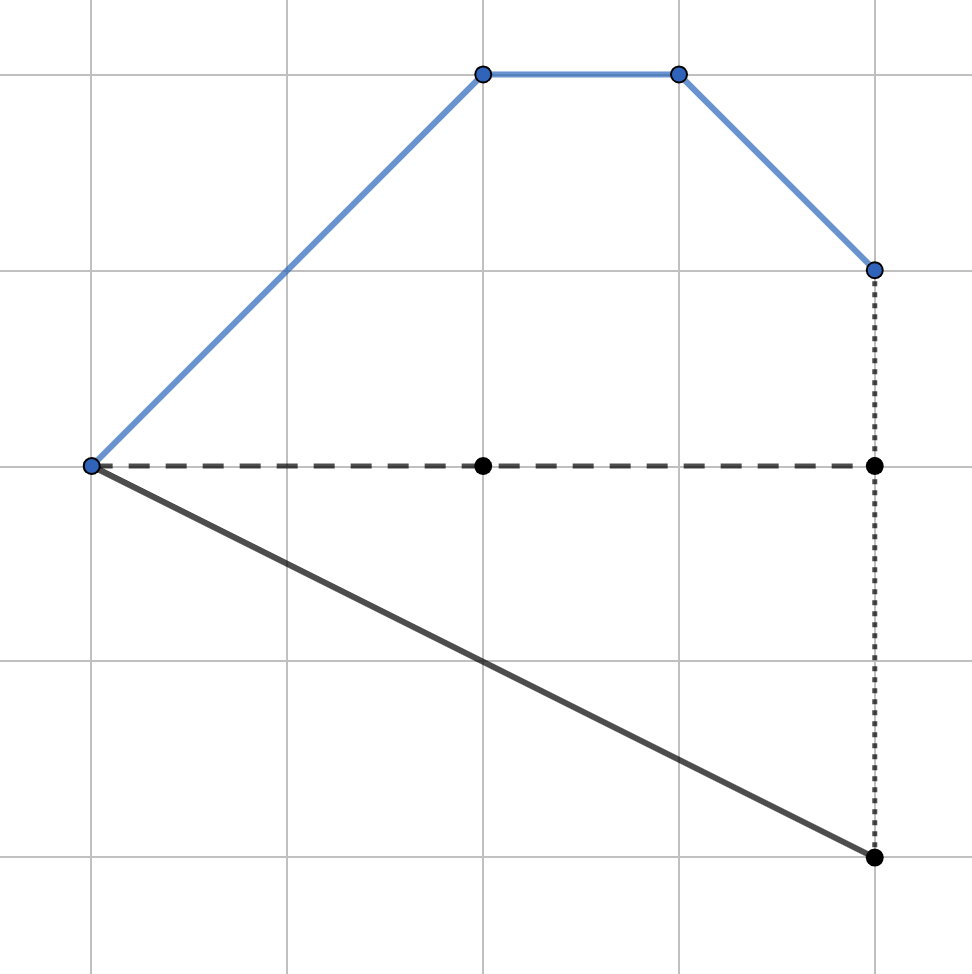
\includegraphics[scale=0.5]{gencdp.png}
  \caption{Пример генерации CDP из многогранника: голубым обозначены ребра, которые войдут в $\psi_1$, черным (сплошным) - ребра, которые войдут в $\psi_2$}\label{correntcdp}
\end{figure}


\noindent{Результат:}
\begin{lstlisting}[style=output]
CDP object, psi list:
Piecewise affine function:
Affine function 3 - x_1 with domain [(1), (2)]
Affine function 2 with domain [(0), (1)]
Affine function 2 + x_1 with domain [(-2), (0)]

Piecewise affine function:
Affine function 2 with domain [(-2), (2)],

base: (A vertex at (-2), A vertex at (2))
\end{lstlisting}



\newgeometry{left=20mm, right=15mm, bottom=20mm}
\section{Приложение}
\fontsize{14}{12}\selectfont
\subsection{piecewise\_affine\_function.py} \label{piece}
\lstinputlisting[language=Python, style=python]{piecewise_affine_function.py}
\clearpage
\subsection{cdp.py} \label{cdppy}
\lstinputlisting[language=Python, style=python]{cdp.py}
\clearpage
\subsection{generate\_cdp.py} \label{gen}
\lstinputlisting[language=Python, style=python]{generate_cdp.py}
\clearpage
\restoregeometry

\clearpage
\printbibliography %Prints bibliography

\end{document}	